\section{Phân phối Nhị thức (Binomial Distribution)}

\subsection{Định nghĩa}

Phân phối nhị thức mô tả xác suất có chính xác $k$ lần \textbf{thành công} trong $n$ phép thử độc lập, 
trong đó mỗi phép thử có xác suất thành công $p$ không đổi.  
Ta ký hiệu:
\[
X \sim \mathrm{Binomial}(n, p), \quad n \in \mathbb{N}, \; 0 \leq p \leq 1
\]


Đặt biệt, các điều kiện sau cần được thỏa:

\begin{itemize}
    \item Số lượng phép thử $n$ là cố định 
    \item Các phép thử là độc lập nhau
    \item Xác suất thành công của từng phép thử là như nhau cho mỗi lần thử
    \item Mỗi phép thử, hoặc là thành công, hoặc là không thành công.
\end{itemize}
\subsection{Probability Mass Function - PMF}

Hàm trọng lượng xác suất của phân phối nhị thức được cho bởi:
\[
P(X = k) = f(k; n, p) = \binom{n}{k} p^k (1 - p)^{n - k}, \quad k = 0, 1, 2, \dots, n
\]
với:
\[
\binom{n}{k} = \frac{n!}{k!(n - k)!}
\]
là hệ số tổ hợp, biểu thị số cách chọn $k$ thành công trong $n$ phép thử.

\subsection{Cumulative Distribution Function - CDF}

Hàm xác suất tích lũy được định nghĩa là:
\[
F(k; n, p) = P(X \leq k) = \sum_{i = 0}^{k} \binom{n}{i} p^i (1 - p)^{n - i}
\]
Không có công thức đóng cho $F(k; n, p)$, nhưng có thể tính xấp xỉ bằng hàm Beta không đều (incomplete Beta function):
\[
F(k; n, p) = I_{1-p}(n - k, k + 1)
\]
  
\begin{figure}[h!]
    \centering
    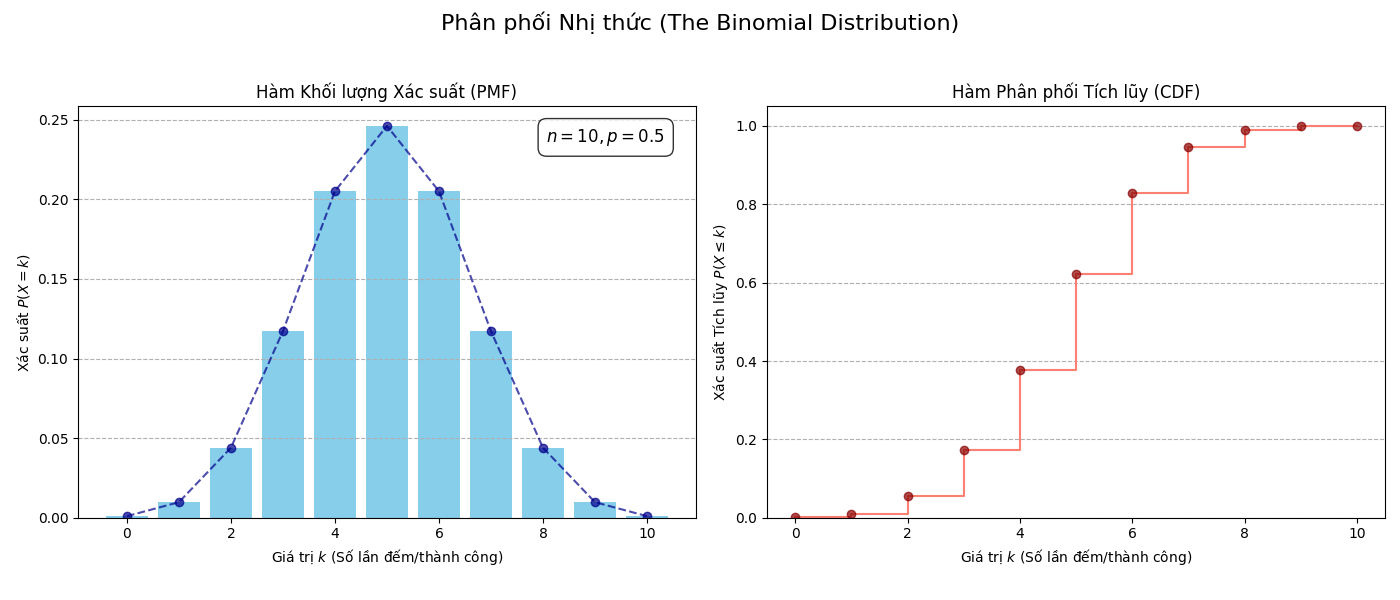
\includegraphics[width=0.8\textwidth]{images/Binomial_PMF_and_CDF.png}
    \caption{Biểu đồ Hàm Khối lượng Xác suất (PMF) và Hàm Phân phối Tích lũy (CDF) của Phân phối Nhị thức. Phân phối này mô tả số lần thành công trong $n$ phép thử độc lập.}
    \label{fig:binomial_dist}
\end{figure}
\subsection{Các đặc trưng thống kê}

\begin{itemize}
    \item \textbf{Giá trị kỳ vọng (Mean):} 
    \[
    \mathbb{E}[X] = np
    \]
    \item \textbf{Phương sai (Variance):} 
    \[
    \mathrm{Var}(X) = np(1 - p)
    \]
    \item \textbf{Mode (Giá trị có xác suất cao nhất):}
    \[
    \mathrm{mode} = \lfloor (n + 1)p \rfloor
    \]
    \item \textbf{Median (Trung vị, xấp xỉ):}
    \[
    \mathrm{median} \approx \lfloor np + \tfrac{1}{2} \rfloor
    \]
    \item \textbf{Miền xác định:}
    \[
    k \in \{0, 1, 2, \dots, n\}
    \]
\end{itemize}

\subsection{Tính chất hình dạng (Shape)}

\begin{itemize}
    \item Phân phối nhị thức là \textbf{đối xứng} nếu $p = 0.5$.  
    \item \textbf{Lệch trái (left-skewed)} nếu $p > 0.5$.  
    \item \textbf{Lệch phải (right-skewed)} nếu $p < 0.5$.  
    \item Khi $n$ lớn và $p$ không quá gần 0 hoặc 1, phân phối nhị thức có thể được \textbf{xấp xỉ bằng phân phối chuẩn (Normal Distribution)} với:
    \[
    X \approx \mathcal{N}(np, \, np(1 - p))
    \]
\end{itemize}

\subsection{Ví dụ dữ liệu và ứng dụng thực tế}

\paragraph{Ứng dụng 1: Kiểm định chất lượng sản phẩm.} 
Với số lượng các sản phẩm cho trước kết hợp với xác suất của một mặt hàng bị lỗi
Phân phối nhị thức có thể giúp xây dựng mô hình và ước lượng số lượng
mặt hàng bị lỗi, điều này giúp các nhà xây dựng sản phẩm cân nhắc về chất lượng
sản phẩm cũng như việc quản lý hệ thống, thiết bị sản xuất.


\paragraph{Ứng dụng 2: Ứng dụng trong tài chính.} 
Phân phối nhị thức đóng vai trò nền tảng trong  
\textit{Binomial Option Pricing Model} – BOPM)  
Thay vì giả định giá tài sản biến thiên liên tục (như trong mô hình Black–Scholes), 
Mô hình này giả định rằng ở mỗi bước thời gian $\Delta t$, giá tài sản cơ sở $S$ chỉ có thể:
\[
S_u = S_0 u \quad \text{hoặc} \quad S_d = S_0 d
\]
tức rằng tăng u lần hoặc là d lần
Sau $( n )$ bước (tức ta chia khoảng thời gian thành n windows và coi nó là rời rạc),
 giá cổ phiếu có thể đi qua nhiều đường khác nhau, ta có thể từ đó quan tâm đến
số lần tăng  k  trong  n  bước.

Xác suất để cổ phiếu tăng đúng  k  lần tuân theo phân phối nhị thức:

$$
P(K = k) = \binom{n}{k} p^k (1 - p)^{n-k}
$$

Từ đó, giá quyền chọn được tính bằng kỳ vọng có trọng số của các giá trị cuối cùng, với trọng số chính là xác suất nhị thức này.

$$
C_0 = e^{-rT} \sum_{k=0}^{n} \binom{n}{k} p^k (1 - p)^{n-k} , \max(u^k d^{n-k} S_0 - K, 0)
$$

Mô hình này cung cấp một cách tiếp cận rời rạc, trực quan và hiệu quả để ước lượng giá trị quyền chọn, 
đồng thời hội tụ về mô hình Black–Scholes khi $n \to \infty$.

\begin{figure}[h!]
    \centering
    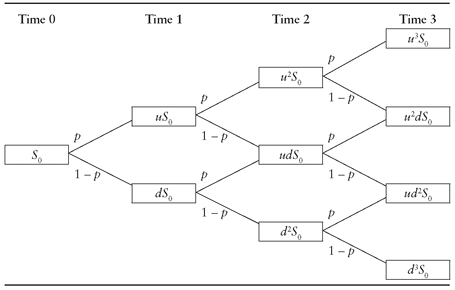
\includegraphics[width=0.8\textwidth]{images/BOCM.png}
    \caption{Cây nhị phân mô tả sự biến động của giá tài sản cơ sở 
    qua ba giai đoạn thời gian trong mô hình định giá quyền chọn nhị thức}
    \label{fig:BOPM}
\end{figure}

\newpage
\section{Phân phối Poisson (Poisson Distribution)}

\subsection{Định nghĩa}

Phân phối Poisson mô tả xác suất của số sự kiện xảy ra trong một khoảng cố định (thời gian, không gian, v.v.),  
nếu các sự kiện xảy ra độc lập và với tốc độ trung bình $\lambda$ không đổi.  
Ký hiệu:
\[
X \sim \mathrm{Poisson}(\lambda), \quad \lambda > 0
\]

\subsection{Probability Mass Function – PMF}

Hàm trọng lượng xác suất của phân phối Poisson là:
\[
P(X = k) = f(k; \lambda) = \frac{\lambda^k e^{-\lambda}}{k!}, \quad k = 0, 1, 2, \dots
\]

\subsection{Cumulative Distribution Function – CDF}

Hàm xác suất tích lũy được định nghĩa là:
\[
F(k; \lambda) = P(X \le k) = \sum_{i=0}^k \frac{\lambda^i e^{-\lambda}}{i!}
\]

\begin{figure}[h!]
    \centering
    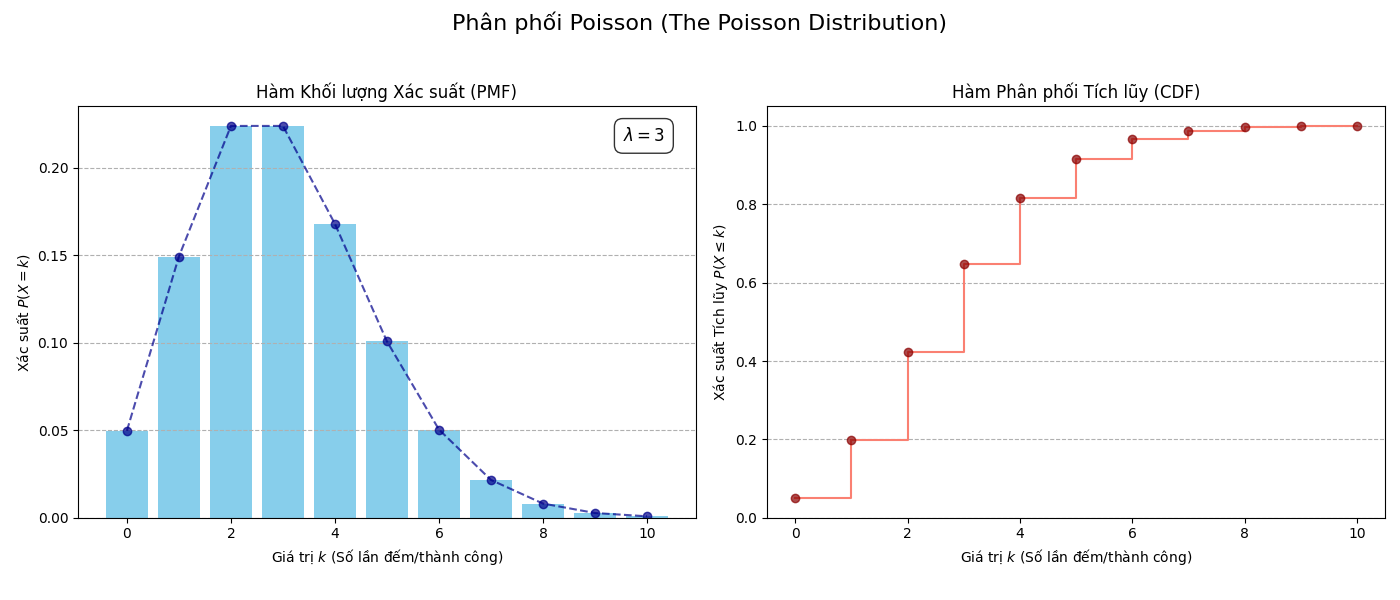
\includegraphics[width=0.8\textwidth]{images/Poisson_PMF_and_CDF.png}
    \caption{Biểu đồ PMF và CDF của Phân phối Poisson. Phân phối này mô hình hóa số sự kiện xảy ra trong một khoảng thời gian/không gian cố định, với tốc độ trung bình ($\lambda$) đã biết.}
    \label{fig:poisson_dist}
\end{figure}
\subsection{Các đặc trưng thống kê}

\begin{itemize}
  \item \textbf{Kỳ vọng (Mean):}  
  \[
    \mathbb{E}[X] = \lambda
  \]
  \item \textbf{Phương sai (Variance):}  
  \[
    \mathrm{Var}(X) = \lambda
  \]
  \item \textbf{Mode (giá trị có xác suất cao nhất):}  
  Nếu $\lambda$ không phải số nguyên, mode = $\lfloor \lambda \rfloor$.  
  Nếu $\lambda$ là số nguyên, thì có hai mode là $\lambda$ và $\lambda - 1$. 
  \item \textbf{Median (Trung vị, xấp xỉ):}  
  Không có công thức đóng chính xác; một xấp xỉ thường dùng là  
  \[
    \mathrm{median} \approx \left\lfloor \lambda + \frac{1}{3} - \frac{1}{50\lambda} \right\rfloor
  \] 
  \item \textbf{Miền xác định:}  
  \[
    k \in \{0, 1, 2, \dots\}
  \]
  \item \textbf{Hình dạng / Độ lệch:}  
  - Phân phối Poisson thường mang lệch phải (right-skewed).  
  - Khi $\lambda$ lớn, phân phối gần đối xứng và có thể xấp xỉ 
  bằng phân phối chuẩn.   
\end{itemize}
\begin{figure}[h!]
    \centering
    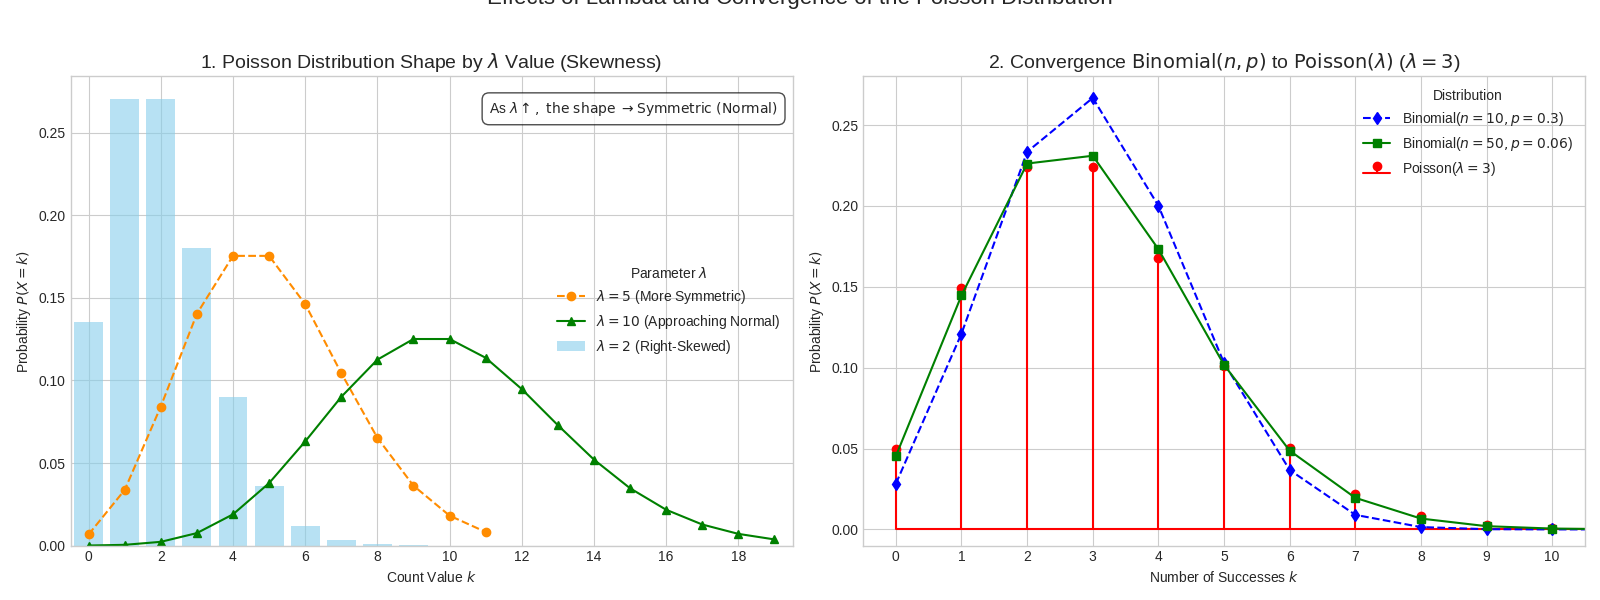
\includegraphics[width=0.8\textwidth]{images/Poisson_Shape_and_Binomial_Convergence.png}
    \caption{Hình dạng của phân phối Possion với các tham số khác nhau.}
    \label{fig:poisson_dist}
\end{figure}
\subsection{Mối liên hệ với phân phối nhị thức}


Khi $n$ rất lớn và $p$ rất nhỏ sao cho $np = \lambda$ không đổi, phân phối nhị thức $\mathrm{Binomial}(n, p)$ hội tụ về phân phối Poisson $\mathrm{Poisson}(\lambda)$:  
\[
\lim_{n \to \infty,\, p \to 0,\; np = \lambda} \binom{n}{k} p^k (1 - p)^{n-k} = \frac{\lambda^k e^{-\lambda}}{k!}
\]

\subsection*{Ví dụ dữ liệu và ứng dụng thực tế }
Phân phối \textbf{Poisson} là công cụ tiêu chuẩn để mô hình hóa 
số lần xảy ra của các sự kiện hiếm và độc lập trong một khoảng thời gian cố định.
Ví dụ, ta có thể xem xét việc số lần nhấp chuột vào một trang quảng cáo/ mặt hàng,...

\textbf{Mục tiêu bài toán là} dự đoán số lần ($X$) một khách hàng nhấp chuột vào quảng cáo trên trang web trong một khoảng thời gian cố định (ví dụ: 5 phút).
 Tỷ lệ nhấp chuột trung bình (mean click rate) trong khoảng thời gian đó.
 Giả định rằng các lần nhấp chuột xảy ra độc lập với một tốc độ không đổi.
Xác suất để xảy ra chính xác $k$ lần nhấp chuột được tính như sau:
    $$
        P(X=k) = (e^{-\lambda} * \lambda^k) / k!
    $$
 \textbf{Điều kiện áp dụng:} Phân phối Poisson chỉ phù hợp nếu
 \textbf{Trung bình gần bằng Phương sai} (Equidispersion). 
 Nếu \textbf{Phương sai lớn hơn cả Trung bình} (Overdispersion), thì
 \textbf{Hồi quy Nhị thức Âm} cần được sử dụng để xử lý sự khác biệt hành vi lớn giữa các khách hàng.

\section{Phân phối Nhị thức Âm}

\subsection{Định nghĩa}

Phân phối Nhị thức Âm mô tả xác suất của số lần \textbf{thất bại} ($k$) xảy ra trước khi đạt được một số lượng \textbf{thành công} cố định là $r$. Phân phối này là một giải pháp quan trọng cho \textbf{dữ liệu đếm (count data)} khi có hiện tượng \textbf{phân tán quá mức (overdispersion)} so với mô hình Poisson.

Ta ký hiệu:
\[
X \sim \mathrm{NegativeBinomial}(r, p), \quad r \in \mathbb{N}^+, \; 0 < p \leq 1
\]
Trong Data Science, nó thường được tham số hóa theo \textbf{kỳ vọng} ($\mu$) và \textbf{tham số phân tán} ($k$ hoặc $\alpha$), nơi $\mathrm{Var}(X) = \mu + \mu^2 / k$.

\subsection{Probability Mass Function - PMF}

Hàm trọng lượng xác suất của phân phối nhị thức âm (số lần thất bại $k$ trước $r$ lần thành công) được cho bởi:
\[
P(X = k) = f(k; r, p) = \binom{k + r - 1}{k} p^r (1 - p)^{k}, \quad k = 0, 1, 2, \dots
\]
với:
\[
\binom{k + r - 1}{k} = \frac{(k + r - 1)!}{k!(r - 1)!}
\]
là hệ số tổ hợp, biểu thị số cách sắp xếp $k$ thất bại và $r$ thành công trong $(k+r)$ phép thử, với phép thử cuối cùng phải là thành công thứ $r$.

\subsection{Cumulative Distribution Function - CDF}

Hàm xác suất tích lũy được định nghĩa là:
\[
F(k; r, p) = P(X \leq k) = \sum_{i = 0}^{k} \binom{i + r - 1}{i} p^r (1 - p)^{i}
\]
Giống như phân phối Nhị thức, CDF của NBD có thể liên hệ với hàm Beta không đều:
\[
F(k; r, p) = I_{p}(r, k + 1)
\]

\begin{figure}[h!]
 \centering
 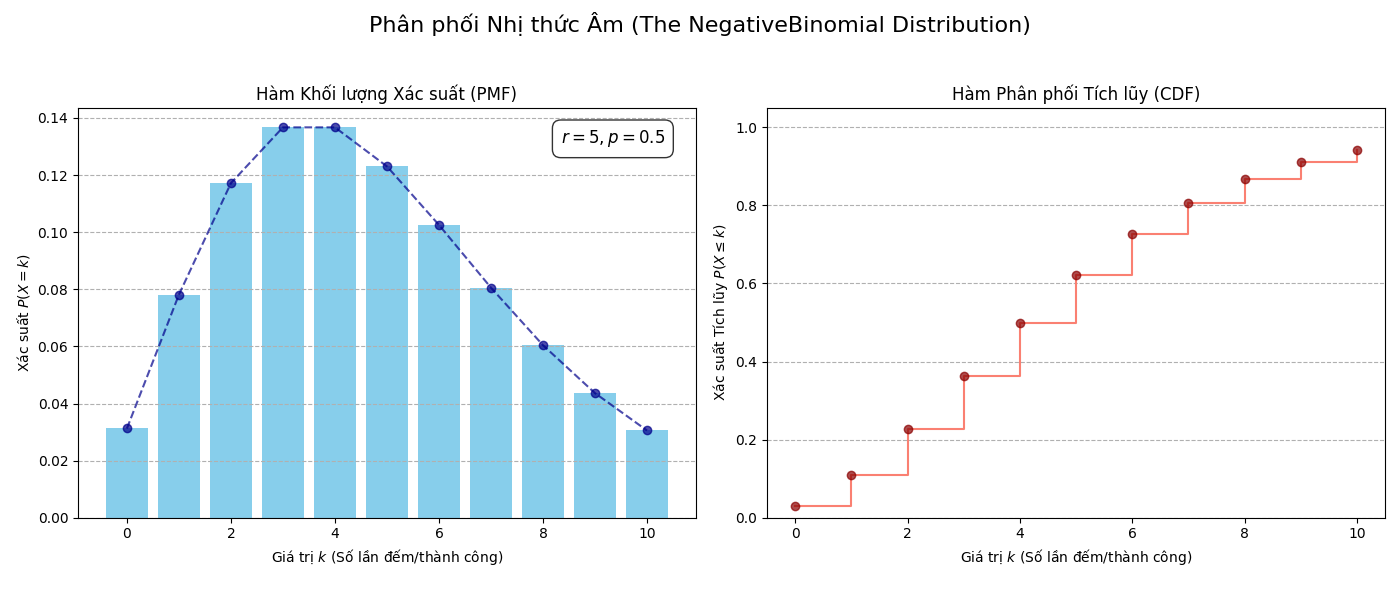
\includegraphics[width=0.8\textwidth]{images/NegativeBinomial_PMF_and_CDF.png}
\caption{Biểu đồ Hàm Khối lượng Xác suất (PMF) và Hàm Phân phối Tích lũy (CDF) của Phân phối Nhị thức Âm. Phân phối này mô tả số lần thất bại trước khi đạt $r$ thành công cố định.}
\label{fig:nbinomial_dist}
\end{figure}

\subsection{Các đặc trưng thống kê}

\begin{itemize}
\item \textbf{Giá trị kỳ vọng (Mean):} 
 $$
\mathbb{E}[X] = \frac{r(1 - p)}{p} = \mu
    $$
\item \textbf{Phương sai (Variance):} 
$$
\mathrm{Var}(X) = \frac{r(1 - p)}{p^2} = \mu + \frac{\mu^2}{r/{(1-p)}} = \mu + \frac{\mu^2}{k_{alt}}
$$
    \textbf{Lưu ý:} Phương sai luôn \textbf{lớn hơn} giá trị kỳ vọng: $\mathrm{Var}(X) > \mathbb{E}[X]$.
\item \textbf{Miền xác định:}
 $$
 k \in \{0, 1, 2, \dots\}
 $$
\end{itemize}

\subsection{Mối liên hệ với các phân phối khác}

\begin{itemize}
\item \textbf{Mở rộng của Hình học (Geometric):} Nếu $r=1$, NBD trở thành Phân phối Hình học (Geometric Distribution), mô tả số lần thất bại trước \textit{thành công đầu tiên}.
\item \textbf{Xấp xỉ Poisson:} Nếu $r \to \infty$ và $p \to 1$ sao cho $\frac{r(1-p)}{p} = \lambda$ không đổi, NBD hội tụ về $\mathrm{Poisson}(\lambda)$.
\end{itemize}

\subsection{Ví dụ dữ liệu và ứng dụng thực tế}

\subsubsection*{Bài toán Dự đoán Tần suất Mua hàng}

\textbf{Mục tiêu bài toán} là xây dựng mô hình dự đoán \textbf{số lần}
một khách hàng cá nhân sẽ thực hiện giao dịch (mua hàng) 
trong một \textbf{khoảng thời gian cố định trong tương lai} 
(ví dụ: 6 tháng, 1 năm).  

Để làm được điều đó, ta sử dụng dữ liệu giao dịch lịch sử của từng khách hàng, bao gồm:

\begin{itemize}
    \item \textbf{Số lần mua hàng ($k$):} Tổng số giao dịch được ghi nhận trong khoảng thời gian quan sát đối với từng khách hàng.
    \item \textbf{Các biến giải thích (Covariates):} Đặc trưng hành vi và nhân khẩu học ảnh hưởng đến tần suất mua hàng — chẳng hạn như \textit{giá trị đơn hàng trung bình}, \textit{thời gian kể từ lần mua gần nhất}, hay \textit{nguồn gốc khách hàng}.
\end{itemize}

\subsubsection*{Vấn đề của Phân phối Poisson} 

Khi áp dụng \textbf{Hồi quy Poisson (Poisson Regression)} để dự đoán tần suất mua hàng,  
người ta thường gặp phải hiện tượng \textbf{phân tán quá mức (Overdispersion)}, tức là 
phương sai của dữ liệu lớn hơn rất nhiều so với giá trị trung bình.  

Nguyên nhân xuất phát từ hai giả định chính của mô hình Poisson:
\begin{itemize}
    \item \textbf{Giả định về phương sai:} Phân phối Poisson yêu cầu $\text{Mean}(\mu) = \text{Variance}(\sigma^2)$.
    \item \textbf{Sự không đồng nhất hành vi:} Trong thực tế, có sự khác biệt rõ rệt giữa nhóm khách hàng “mua thường xuyên” và nhóm “mua ngẫu nhiên”.  
    Điều này khiến phương sai quan sát được trong dữ liệu lớn hơn nhiều so với trung bình, vi phạm giả định cơ bản của Poisson.
\end{itemize}

\subsubsection*{Giải pháp: Sử dụng Phân phối Nhị thức Âm (Negative Binomial Distribution)}

Để xử lý hiện tượng \textit{overdispersion}, ta sử dụng phân phối Nhị thức Âm (NBD),
vốn là sự mở rộng của Poisson khi cho phép phương sai linh hoạt hơn.  

Phân phối này có thể được hiểu như một \textbf{mô hình hợp (compound model)} giữa hai phân phối:

\begin{itemize}
    \item \textbf{Phân phối Poisson:} Mô tả số lần mua hàng của một cá nhân, giả sử tốc độ mua hàng của họ là $\lambda$ cố định.
    \item \textbf{Phân phối Gamma:} Mô hình hóa sự biến thiên ngẫu nhiên của $\lambda$ giữa các cá nhân (tức là sự không đồng nhất trong hành vi mua hàng giữa khách hàng này với khách hàng khác).
\end{itemize}

\begin{figure}[h!]
    \centering
    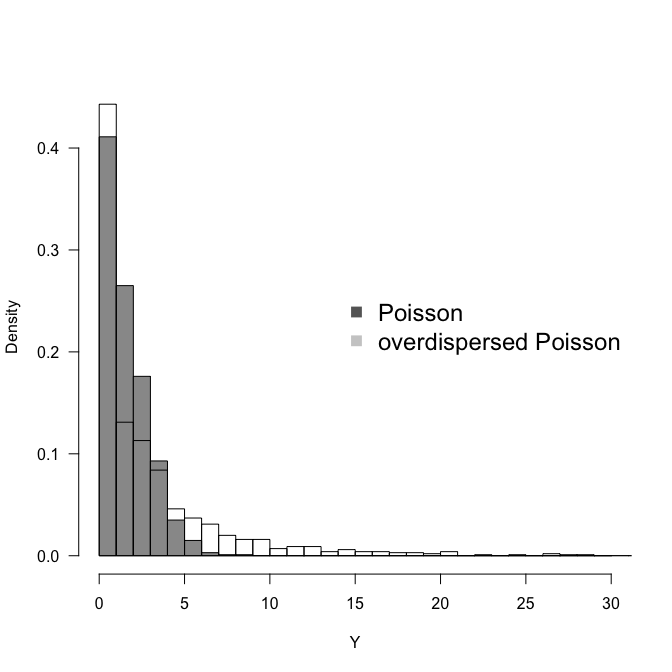
\includegraphics[width=0.85\textwidth]{images/Overdispersion_pois.png}
    \caption{So sánh giữa phân phối Poisson chuẩn và Poisson có hiện tượng \textbf{overdispersion} (phương sai lớn hơn trung bình). 
    Dữ liệu xám đậm thể hiện phân phối Poisson với tham số $\lambda = 2$, 
    trong khi dữ liệu xám nhạt biểu diễn phân phối Poisson bị overdispersed với $\lambda$ thay đổi ngẫu nhiên theo $2 e^{Z}$, $Z \sim \mathcal{N}(0, 1)$.}
    \label{fig:poisson_overdispersion}
\end{figure}
Khi ta \textbf{tích hợp (marginalize)} $\lambda$ theo phân phối Gamma, 
ta thu được phân phối Nhị thức Âm cho số lần mua hàng $X$:

\[
X \sim \mathrm{NegBinomial}(r, p)
\]

với kỳ vọng và phương sai được biểu diễn là:
\[
\mathbb{E}[X] = \mu, \qquad
\mathrm{Var}(X) = \mu + \frac{\mu^2}{k}
\]

Trong đó:
\begin{itemize}
    \item $\mu$ là giá trị trung bình kỳ vọng của số lần mua hàng.
    \item $k$ (hoặc $\alpha$) là \textbf{tham số phân tán (dispersion parameter)}.  
    Khi $k \to \infty$, phương sai tiệm cận $\mu$, và phân phối Nhị thức Âm hội tụ về phân phối Poisson.
\end{itemize}

Nhờ có tham số phân tán này, mô hình Negative Binomial linh hoạt hơn Poisson,  
cho phép mô hình hóa chính xác hành vi mua hàng thực tế, nơi phương sai thường vượt xa trung bình.


\section{Phân phối Đa thức (Multinomial Distribution)}

\subsection{Định nghĩa}

Phân phối \textbf{Đa thức} là sự mở rộng tự nhiên của phân phối Nhị thức (Binomial Distribution),  
được dùng để mô tả xác suất của các kết quả thuộc nhiều hơn hai loại,  
trong $n$ lần thử độc lập, mỗi lần thử có $k$ khả năng xảy ra tương ứng với các xác suất $p_1, p_2, \dots, p_k$ (với $\sum_{i=1}^{k} p_i = 1$).  

Ký hiệu:
\[
(X_1, X_2, \dots, X_k) \sim \mathrm{Multinomial}(n; p_1, p_2, \dots, p_k)
\]
với điều kiện $\sum_{i=1}^{k} X_i = n$.

\subsection{Probability Mass Function – PMF}

Hàm trọng lượng xác suất của phân phối Đa thức là:
\[
P(X_1 = x_1, X_2 = x_2, \dots, X_k = x_k) 
= \frac{n!}{x_1! \, x_2! \, \dots \, x_k!} 
\prod_{i=1}^{k} p_i^{x_i},
\quad \text{với } \sum_{i=1}^{k} x_i = n
\]

\subsection{Cumulative Distribution Function – CDF}

Không có biểu thức đóng cho CDF của phân phối Đa thức.  
Tuy nhiên, ta có thể tính xác suất cộng dồn bằng cách lấy tổng các giá trị PMF cho tất cả các tổ hợp $\{x_i\}$ thỏa $\sum_i x_i \le m$:
\[
F(m; n, \mathbf{p}) = P\left(\sum_{i=1}^{k} X_i \le m\right) = 
\sum_{\substack{x_1 + \dots + x_k \le m}} 
\frac{n!}{x_1! \, x_2! \, \dots \, x_k!} 
\prod_{i=1}^{k} p_i^{x_i}
\]

% \begin{figure}[h!]
%     \centering
%     \includegraphics[width=0.85\textwidth]{images/Multinomial_Distribution_Simplex.png}
%     \caption{Minh họa phân phối Multinomial cho $k=3$ loại kết quả khác nhau. Các giá trị $(x_1, x_2, x_3)$ thỏa $\sum x_i = n$ tạo thành một \textbf{simplex} trong không gian xác suất.}
%     \label{fig:multinomial_dist}
% \end{figure}

\subsection{Các đặc trưng thống kê}

\begin{itemize}
  \item \textbf{Kỳ vọng (Mean):}  
  \[
    \mathbb{E}[X_i] = n p_i, \quad i = 1, \dots, k
  \]
  \item \textbf{Phương sai (Variance):}  
  \[
    \mathrm{Var}(X_i) = n p_i (1 - p_i)
  \]
  \item \textbf{Hiệp phương sai (Covariance):}  
  \[
    \mathrm{Cov}(X_i, X_j) = -n p_i p_j, \quad i \ne j
  \]
  \item \textbf{Miền xác định:}  
  \[
    x_i \in \{0, 1, \dots, n\}, \quad \sum_{i=1}^{k} x_i = n
  \]
  \item \textbf{Hình dạng:}  
  - Phân phối này luôn nằm trong miền đơn hình (simplex).  
  - Khi $n$ lớn, phân phối Multinomial có thể được xấp xỉ bởi phân phối Chuẩn đa biến:
  \[
  \mathbf{X} \sim \mathcal{N}\big(n\mathbf{p},\, n(\mathrm{diag}(\mathbf{p}) - \mathbf{p}\mathbf{p}^T)\big)
  \]
\end{itemize}

\subsection*{Ứng dụng: Mô hình Hóa Phân Bố Từ Ngữ trong Văn Bản}

Một ứng dụng nổi bật của \textbf{phân phối Multinomial} là trong mô hình \textbf{Bag-of-Words (BoW)} trong xử lý ngôn ngữ tự nhiên (NLP).  
Giả sử ta có một từ điển gồm $k$ từ khác nhau, và một văn bản chứa tổng cộng $n$ từ.  
Nếu ta coi mỗi từ trong văn bản được chọn ngẫu nhiên và độc lập với xác suất $p_i$ (xác suất xuất hiện của từ thứ $i$ trong ngôn ngữ),  
thì số lần xuất hiện $(X_1, X_2, \dots, X_k)$ của các từ đó trong văn bản tuân theo:
\[
(X_1, X_2, \dots, X_k) \sim \mathrm{Multinomial}(n; p_1, p_2, \dots, p_k)
\]

Ví dụ, trong mô hình \textbf{Naive Bayes phân loại văn bản},  
ta giả định rằng xác suất xuất hiện của các từ trong một tài liệu thuộc lớp $C_j$ được mô hình hóa bởi tham số $\mathbf{p}^{(j)} = (p_1^{(j)}, \dots, p_k^{(j)})$.  
Với một tài liệu có vector tần suất từ $\mathbf{x} = (x_1, \dots, x_k)$,  
ta có:
\[
P(\mathbf{x} \mid C_j) = \frac{n!}{x_1! \cdots x_k!} 
\prod_{i=1}^{k} \big(p_i^{(j)}\big)^{x_i}
\]
và xác suất hậu nghiệm theo định lý Bayes:
\[
P(C_j \mid \mathbf{x}) = \frac{P(C_j) \, P(\mathbf{x} \mid C_j)}{\sum_{l} P(C_l) \, P(\mathbf{x} \mid C_l)}
\]

\textbf{Ảnh hưởng thực tế:}  
Nhờ giả định Multinomial, mô hình Naive Bayes có thể ước lượng trực tiếp 
xác suất từ vựng của từng lớp dựa trên tần suất xuất hiện từ trong dữ liệu huấn luyện,  
cho phép phân loại tài liệu hiệu quả và có cơ sở xác suất chặt chẽ.  
Phân phối Multinomial đóng vai trò nền tảng trong việc định nghĩa hàm khả năng (likelihood) của văn bản trong nhiều mô hình ngôn ngữ thống kê.

% \begin{figure}[h!]
%     \centering
%     \includegraphics[width=0.85\textwidth]{images/Multinomial_Text_Model.png}
%     \caption{Mô hình Multinomial trong phân loại văn bản: Mỗi tài liệu được xem là tập hợp của $n$ từ, rút ra độc lập từ phân phối $p_i$ đặc trưng cho lớp.}
%     \label{fig:multinomial_text_model}
% \end{figure}
